\section{Emergent Behaviour}

The implementation of the research component began at the end of the first term. At first, a prototype implementation of the algorithm presented in Griffiths 2008 was implemented in Java. This was completed before the end of the first term. The purpose of this implementation was to check that the results in the paper could be replicated, to check that an implementation in Java was feasible and to gain a better understanding of the algorithms. This implementation was completed before the end of the first term.

This implementation was used to ensure that we had a good understanding of how the algorithms in the original paper worked, and to this effect was successful. We found that we had made a couple of incorrect assumptions based on the original paper, such as using directed edges, where the original undirected edges. 

The code for this prototype implementation is available on the attached CD.

The prototype implementation did not allow changes to be made easily. We decided that over the second term we would start anew and re-write the Java code in order to provide a better implementation which was more amenable to adding new functionality.

In the second term, we started to write the final implementation. We decided to base the graph on JUNG for the reasons mentioned in the design section. In this implementation, agents are represented as vertices in the JUNG graph. In order to facilitate this, we had to write a custom subclass to the Apache Factory interface to generate new agents in the graph.

The basic algorithm is run over a number of iterations (generations). In each iteration, the donation phase is run, followed by the reproduction algorithm. These algorithms were designed to allow the user to provide an instance of an object which will provide some of the key features such as rewiring.

A system diagram representing the key data structures and how they interact is shown in figure \ref{fig:graphdatastructures}. The entire system is encapsulated by a instance of the SimGraph class. This class contains an instance of a JUNG graph. Each vertex in this graph is an instance of the Agent class, which is itself an instance of the Vertex class. Each Agent has a unique identifier which is used to access the isObserving and isBeingObservedBy data structures. These data structures are used to handle the observations each agent makes of its neighbouring agents. Each agent can be observing multiple agents therefore, these lookups return a mapping of agents that the agent is observing to the instance of the Observer class that stores the observations the observer made on that agent. The Observer class encapsulates a queue data structure of boolean observations. The two observing data structures, isObserving and isBeingObservedBy are used to provide access to the Observer instances quickly. When a donation is being made, the observations can be quickly added using the isBeingObservedBy data structure, where the isObserving data structure allows the context assessment to be calculated quickly. Two methods, registerObserver and deregisterObserver are used to quickly manipulate the isObserving and isBeingObservedBy data structures, these operations are called during the rewiring operation, as the neighbourhoods and therefore the observers change as a result of the rewiring operation.
The SimGraph class offers a delegate interface, GraphDelegate. The graph instances call methods on a delegate which implements this interface, and is used to notify the delegate of changes to the graph, such as edges being added or removed. It is in these methods that the isObserving and isBeingObservedBy data structures are modified.

\begin{figure}[htbp]
	\centering
	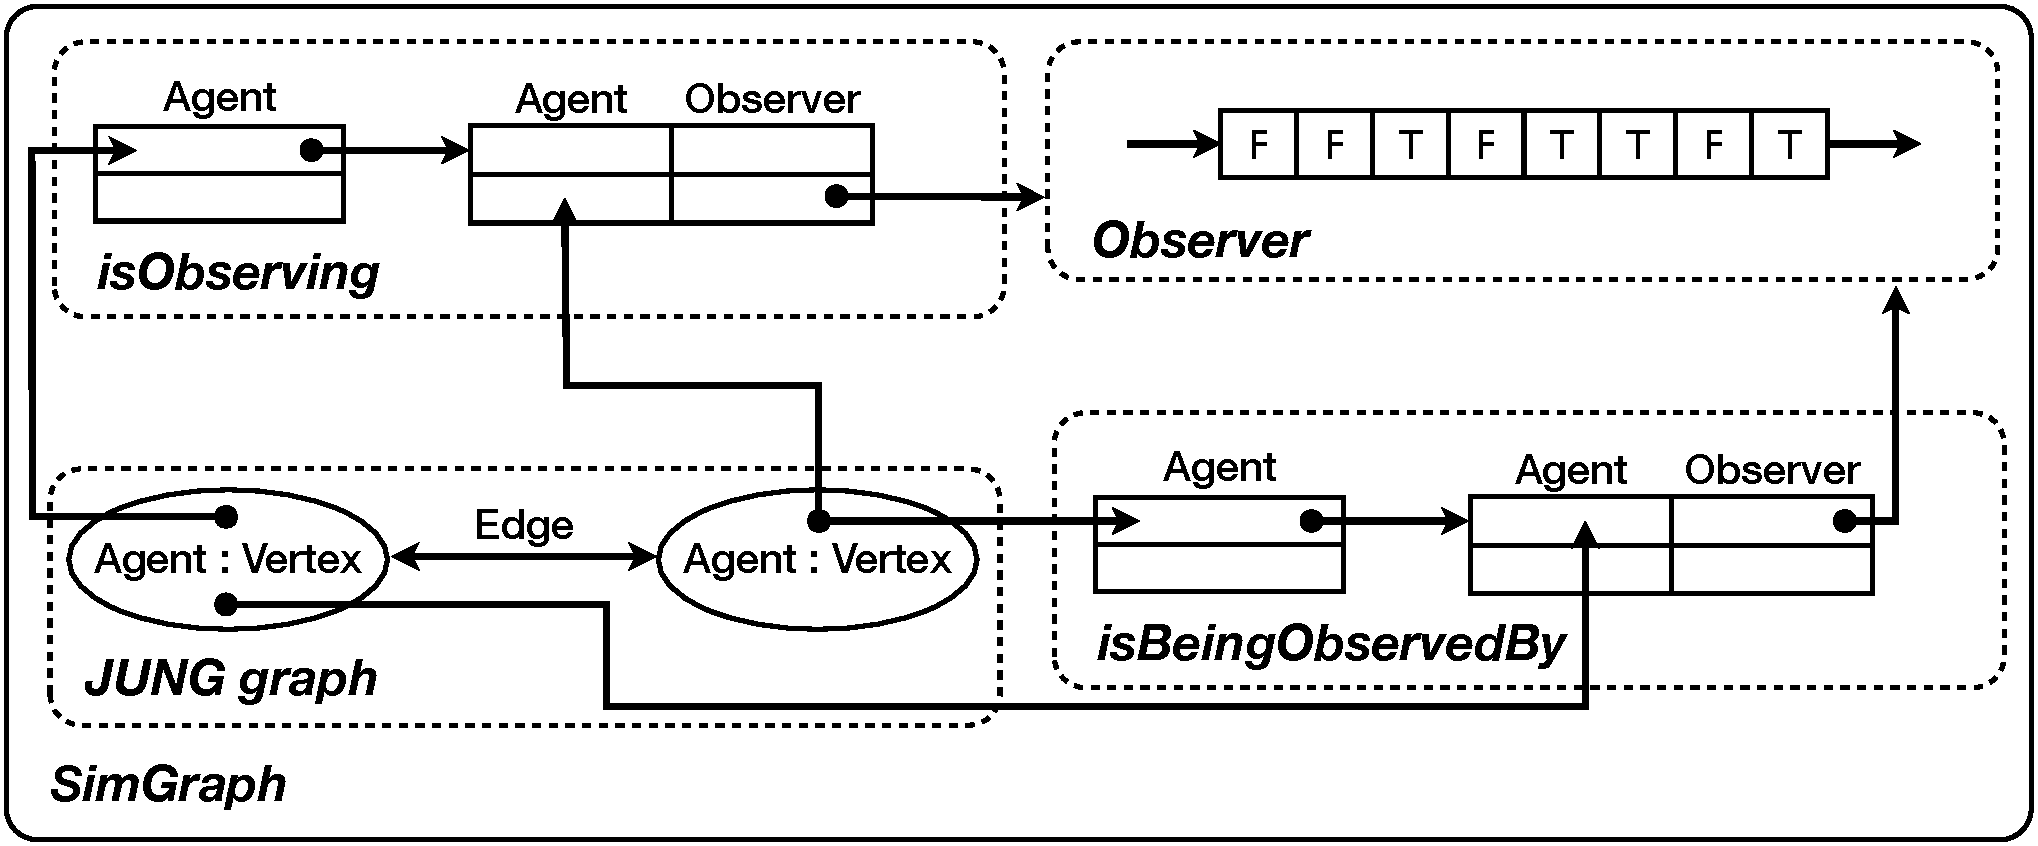
\includegraphics[width=\linewidth]{img/GraphDataStructure.pdf}
	\caption{Graph Data Structures}
	\label{fig:graphdatastructures}
\end{figure}

The donation algorithm used is presented in figure \ref{fig:donationalgorithm}. The main loop runs once for each interaction pairing per generation. In each iteration, every agent is selected (agent A). A random neighbour of agent A is selected (agent B). The tag and tolerances are compared along with the context assessment to determine if agent A will donate to agent B. If agent A has chosen to donate to agent B, then agent A will incur the cost of donating which agent B will gain the benefit of receiving a donation. Once the choice to donate has been made, every observer of agent A will be informed of agent A’s decision to donate or not to donate. After every agent has had the opportunity to donate once for each interaction pairing per generation, the donation phase is complete.

\begin{figure}[htbp]
	\begin{algorithmic}
		\State pairings remaining = interaction pairings per generation
		\While{pairings remaining $> 0$}
			\ForAll{agent $\in$ Graph.vertices}
				\State neighbours = agent.neighbours()
				\State random neighbour = neighbours.random()
				\State will donate = agent.shouldDonateTo(random neighbour)
				\If {will donate = true}
					\State agent.score = agent.score - cost
					\State random neighbour.score = random neighbour.score + benefit
				\EndIf
				\State observeDonation(agent, random neighbour, will donate)
			\EndFor
		\EndWhile
	\end{algorithmic}
	\caption{Donation Algorithm}
	\label{fig:donationalgorithm}
\end{figure}

The learning algorithm is presented in figure \ref{fig:learningalgorithm}. Every agent is selected (agent A). Agent A will select a random agent (agent B) at random. Agent A compares his score to the score of Agent B. If Agent A has a higher score than Agent B, then no learning takes place and the loop continues to the next iteration. If Agent A has a lower score than Agent B, i.e. Agent B is more successful than Agent A, then Agent A will learn from Agent B. Agent A adopts Agent B’s tag and tolerance, with a possibility of donation. After this, Agent A will then use the current rewiring algorithm to rewire its local neighbourhood. Once every agent has had the chance to learn, the learning phase is complete.

\begin{figure}[htbp]
	\begin{algorithmic}
		\ForAll {Agent $\in$ Graph.vertices}
			\State random agent = Graph.random vertex()
			\If {random agent.score > agent.score}
				\State agent.tag = mutate(random agent.score, mutation probability)
				\State agent.tolerance = mutate(random agent.tolerance, mutation probability)
				\State agent.rewire()
			\EndIf
		\EndFor
	\end{algorithmic}
	\caption{Learning Algorithm}
	\label{fig:learningalgorithm}
\end{figure}

At this point, the donation and learning phases have complete, and the single generation has occurred. The donation rate during this donation is calculated using the formula number of donations/opportunities to donate, and these values are reset for the next generation. The calculated donation rates are appended to a comma-separated file database, which can be easily loaded into a spread sheet for examining the results.

Before each simulation, the graphs are generated using the JUNG random graph generating algorithms.

Parameters are loaded into each simulation using an instance of the Parameters class.

The following provides a short description of each class in each
package.

\begin{itemize}
    \item {\tt sim}

    \begin{description}
        \item[Sim] The application entry point, sets the parameters and
        runs a simulation.
    \end{description}

    \item {\tt sim.generators}

    \begin{description}
        \item[GraphGenerator] Abstract base class, used to generate
        graphs.
        \item[RandomGenerator] Extends {\tt GraphGenerator}, creates a
        random graph using an {\it Erdos-Renyi Generator}. Requires
        target vertex and edge counts.
        \item[ScaleFreeGenerator] Extends {\tt GraphGenerator}, creates
        a scale-free graph using a {\it Barabasi-Albert Generator}.
        Requires the initial vertex count, the number of edges to add per
        timestep, and the number of timesteps.
        \item[SmallWorldGenerator] Extends {\tt GraphGenerator}, creates
        a small-world graph using a {\it Kleinberg Generator}.
        Required the lattice size, the number of long distance connections,
        and the clustering exponent.
    \end{description}

    \item {\tt sim.io.graphml}

    \begin{description}
        \item[GraphMLReader] Reads graphs from GraphML files.
    \end{description}

    \item {\tt sim.model}

    \begin{description}
        \item[Observer] Records an Agent's observations of another
        Agent.
        \item[Parameters] Stores the parameters of a simulation.
    \end{description}

    \item {\tt sim.model.edge}

    \begin{description}
        \item[Edge] Empty class---used to represent edges in the graph
    \end{description}

    \item {\tt sim.model.graph}

    \begin{description}
        \item[GraphDelegate] An interface defining methods which can be
        used to respond to changes to the graph.
        \item[GraphType] Abstract base type, used to specify the nature
        of the graph to generate in a simulation.
        \item[RandomGraph] Extends {\tt GraphType}.
        \item[ScaleFreeGraph] Extends {\tt GraphType}.
        \item[SmallWorldGraph] Extends {\tt GraphType}.
        \item[SimGraph] Wrapper around the {\sc jung} {\tt Graph} class.
        Provides notifications to a delegate object of changes to the
        underlying graph.
    \end{description}

    \item {\tt sim.model.rewiring}

    \begin{description}
        \item[RewireStrategy] Abstract base class for rewiring
        algorithms. Provides methods to rank neighbours and perform
        basic rewiring operations.
        \item[RandomRewire] Extends {\tt RewireStrategy}, implements the
        Random rewiring algorithm.
        \item[RandomReplaceWorstRewire] Extends {\tt RewireStrategy},
        implements the \newline Random-Replace-Worst rewiring algorithm.
        \item[IndividualReplaceWorstRewire] Extends {\tt
        RewireStrategy}, implements the \newline Individual-Replace-Worst
        rewiring algorithm.
        \item[GroupReplaceWorstRewire] Extends {\tt RewireStrategy},
        implements the Group-Replace-Worst rewiring algorithm.
    \end{description}

    \item {\tt sim.model.vertex}

    \begin{description}
        \item[Vertex] Used as a vertex in the {\sc jung} graph.
        \item[Agent] Extends {\tt Vertex}, used to store data about each
        agent, such as the tag and tolerance.
        \item[VertexFactory] Used to generate new {\tt Agent} objects as
        Vertices in the graph, allows lookup of generated {\tt Agent}
        instances by id.
    \end{description}

    \item {\tt sim.simulation}

    \begin{description}
        \item[Agents] Keeps track of all the agents in a graph, along
        with their observations.
        \item[DonateAlgorithm] Implementation of the donation phase.
        \item[LearnAlgorithm] Implementation of the learning phase.
        \item[Simulation] Main code for the simulation, takes a set of
        parameters, generates the graph and initial state of the
        simulation, and then runs the simulation.
    \end{description}

    \item {\tt sim.util}

    \begin{description}
        \item[RNG] A singleton subclass of java's {\tt Random} class.
    \end{description}

\end{itemize}
